\section{Second Exercise}
\subsection*{(a)}
\paragraph{Solution:} Consulting Feynman's lectures of physics the energy stored in a uniformly charged sphere is
\begin{equation}
    E = \frac{3}{5} \frac{Q^2}{4 \pi \epsilon_0 R}
\end{equation}
where $Q$ is the total charge, $\epsilon$ is the vacuum permittivity, and $R$ is the radius of the sphere. Since $R = r_0 A^{1/3}$ the equation may be written as
\begin{equation}
        E = \frac{3}{5} \frac{Q^2}{4 \pi \epsilon_0 A^{1/3}} \frac{1}{r_0}.
\end{equation}
The energy difference 
\begin{equation}
    \Delta E = [M(A, Z) - M(A, Z - 1)]c^2\label{eq:MassE}
\end{equation}
may then be written as 
\begin{align}
    \Delta E &= \frac{3}{5} \frac{Z^2 e^2}{4 \pi \epsilon_0 A^{1/3}} \frac{1}{r_0} - \frac{3}{5} \frac{(Z-1)^2 e^2}{4 \pi \epsilon_0 A^{1/3}} \frac{1}{r_0} = \frac{3}{5} \frac{e^2}{4\pi \epsilon_0 A^{1/3}} \frac{1}{r_0} [Z^2 - (Z-1)^2]\\
    =& \frac{3}{5} \frac{(2Z - 1) e^2}{4\pi\epsilon_0 A^{1/3}} \frac{1}{r_0}.
\end{align}
Since $N = Z-1$ we get that $A = 2Z - 1$ which then makes
\begin{equation}
    \Delta E = \frac{3 e^2 A^{2/3}}{20 \pi \epsilon_0} \frac{1}{r_0}.
\end{equation}

\paragraph{Answer:} The relationship between the energy difference and $1/r_0$ is 
\begin{equation}
    \Delta E = \frac{3 e^2 A^{2/3}}{20 \pi \epsilon_0} \frac{1}{r_0}.\label{eq:deltaE}
\end{equation}

\subsection*{(b)}
\begin{table}[H]
    \centering
    \begin{tabular}{ccc|ccc}
    \toprule
         $\nuc{X}{A}{Z}$ & Mass excess [\unit{\micro u}] & $\Delta E$ [MeV] & $\nuc{X}{A}{Z}$ & Mass excess [\unit{\micro u}] & $\Delta E$ [MeV]\\
    \midrule
         $\nuc{B}{11}{5}$   & \num{9305}	& \multirow{2}{*}{933.48}	& $\nuc{N}{15}{7}$	& \num{109}		& \multirow{2}{*}{934.25}	\\
         $\nuc{C}{11}{6}$   & \num{11434}   &						& $\nuc{O}{15}{8}$  & \num{3065}	&						\\
    \midrule
         $\nuc{F}{19}{9}$   & \num{-1597}   & \multirow{2}{*}{934.74}	& $\nuc{Na}{23}{11}$ & \num{-10230}	& \multirow{2}{*}{935.56}	\\
         $\nuc{Ne}{19}{10}$ & \num{1880}    &						& $\nuc{Mg}{23}{12}$ & \num{-5875}	&						\\
    \midrule
         $\nuc{Si}{29}{14}$ & \num{-23505}  & \multirow{2}{*}{936.44}	& $\nuc{Cl}{35}{17}$ & \num{-31147}	& \multirow{2}{*}{937.47}	\\
         $\nuc{P}{29}{15}$  & \num{-18199}  &						& $\nuc{Ar}{35}{18}$ & \num{-24743}	&						\\
    \midrule
         $\nuc{Ca}{41}{20}$ & \num{-37722}  & \multirow{2}{*}{938.00}	& $\nuc{Ti}{45}{22}$ & \num{-41876}	& \multirow{2}{*}{938.63}	\\
         $\nuc{Sc}{41}{21}$ & \num{-30749}  &						& $\nuc{V}{45}{23}$ & \num{-34218}	&						\\
    \bottomrule
    \end{tabular}
    \caption{The error is generally less than $\SI{1}{\micro u}$, so this is the uncertainty that will be used in the error calculations. The calculation of $\Delta E$ according to Eq. \eqref{eq:MassE} and the conversion to MeV is done in the code in App. \ref{app:2cd}.}
    \label{tab:Nuclides}
\end{table}

\subsection*{(c) \& (d)}
\paragraph{Solution:} Rewriting Eq. \eqref{eq:deltaE} with $X = (3 e^2 A^{2/3})/(20 \pi \epsilon_0)$ as
\begin{equation}
    \Delta E = \frac{1}{r_0} X,
\end{equation}
then by calculating $\Delta E$ from Tab. \ref{tab:Nuclides} and Eq. \eqref{eq:MassE} and doing a linear regression and plotting the result gives $r_0 = \SI{1.28}{\femto\m} \pm \SI{0.06}{\femto\m}$ with a $\SI{95.4}{\percent}$ confidence rating. From the lectures we know that $r_0 \approx \SI{1.2}{\femto\m}$, and the calculated value seems reasonable. However, the y-intercept is not at $y=0$ which is a bit weird. 

\begin{figure}[ht]
    \centering
    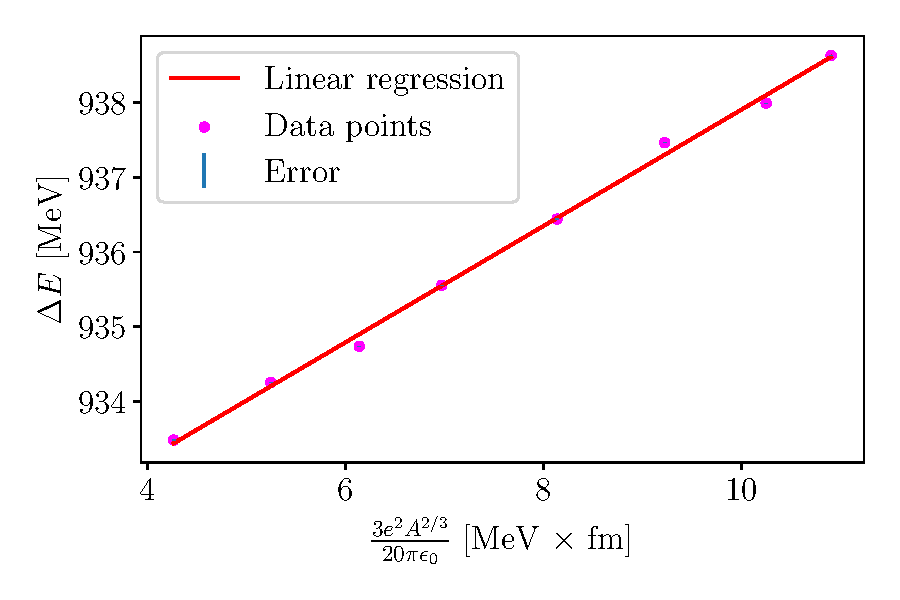
\includegraphics[width=0.8\textwidth]{figures/r0.pdf}
    \caption{Data points and a linear regression. The error bars are not visible since they are smaller than the scatter-markers. For the code see App. \ref{app:2cd}.}
    \label{fig:r0}
\end{figure}

\paragraph{Answer:} The value of $r_0$ is $r_0 = \SI{1.28}{\femto\m} \pm \SI{0.06}{\femto\m}$